\section{Versuchsdurchführung und Auswertung}

\subsection{Verbleibende Aktivität}

Die 22-Na Probe wurde laut Beschriftung am Versuchsaufbau am 29.09.1993 eingesetzt. Sie hatte damals eine Aktivität von $A_{93} = 3,7\e{6} Bq$ und die Halbwertszeit wird mit $t_{\frac{1}{2}} = 2,6 a$ angegeben. Somit ergibt sich für die Restaktivität:
\begin{eqnarray*}
 A(t) = & A_{93} * e^{-\frac{\ln 2}{t_\frac{1}{2}} t} \\
      \approx & 3,61\e{4} Bq
\end{eqnarray*}
Die Messungen in der Staatsexamensarbeit wurden bei $A_{St} = 0,15 mCurie = 5,55\e{6} Bq$ durchgeführt. Wir erwarten also dass die Rate der Ereignisse im Experiment bei uns in etwa zwei Größenordnungen kleiner sein wird. Für die statistische Genauigkeit der Messungen ist dies nicht von Vorteil.

\subsection{Szintillatorspektren}
Wir haben das Spektrum des 22Na mit jedem der drei Szintillatoren aufgenommen (siehe Abb. \ref{22na-schrottspektrum}). Dazu haben wir je einen direkt an den Multi Channel Analysator (MCA) angeschlossen und 20 min gemessen.

\begin{figure}
 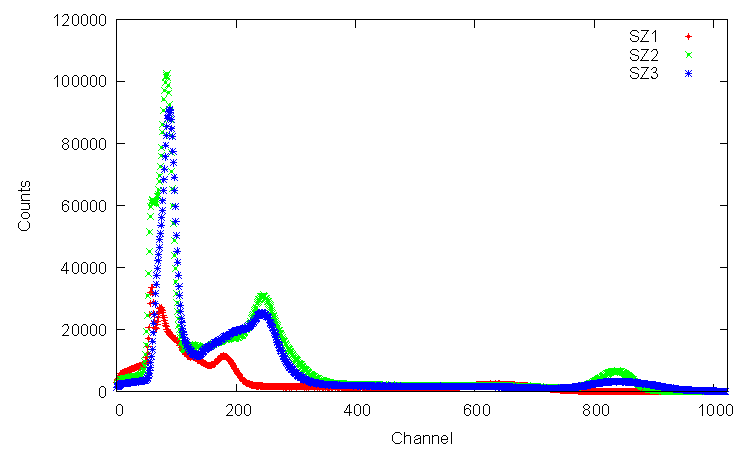
\includegraphics[width=\textwidth]{Graphen/Na-Spektren/na-spektren-1.pdf}
 \caption{Spektrum des 22Na Zerfalls, aufgenommen mit drei ungefilterten Szintilatoren}
 \label{22na-schrottspektrum}
\end{figure}


Bei dem kleineren Peak mit hoher Energie (ca. Channel 850) handelt es sich nicht, wie von uns zuerst vermutet, um die 1270keV Gamma-Quanten des 22Ka-Zerfalls. Vielmehr scheint es sich um einen von der Elektronik erzeugten Störeffekt zu handeln. Der Peak mit der zweithöchsten Energie (Ch.250 bzw. 180) ist dann der eigentliche 1270keV Peak. Die 511keV des Zwei-Photonen-Zerfalls, die Photonen des 3er-Zerfalls und die Bremsstrahlung sind nur schlecht aufgelöst (SZ1 und SZ2) bzw. gar nicht unterscheidbar (SZ3).

Da wir außerdem beim Zuschalten des Single Channel Analysators (SCA) eine Verschiebung des Spektrums beobachteten, haben wir die Energiekalibration dann mit diesem durchgeführt.
\begin{figure}
 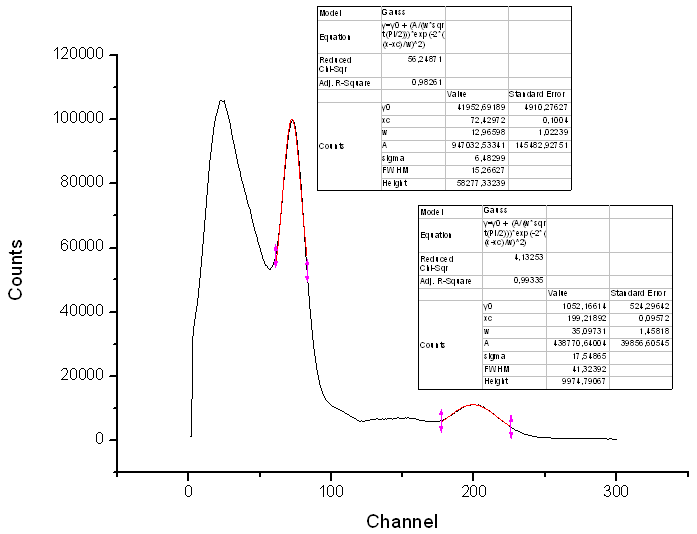
\includegraphics[width=\textwidth]{Graphen/SZ1.png}
 \caption{22Na Spektrum mit SZ1}
\end{figure}

\begin{figure}
 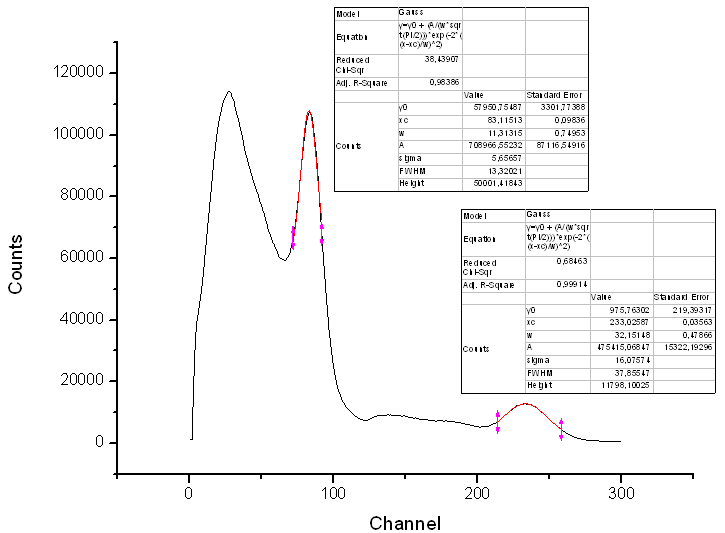
\includegraphics[width=\textwidth]{Graphen/SZ2.png}
 \caption{22Na Spektrum mit SZ2}
\end{figure}

\begin{figure}
 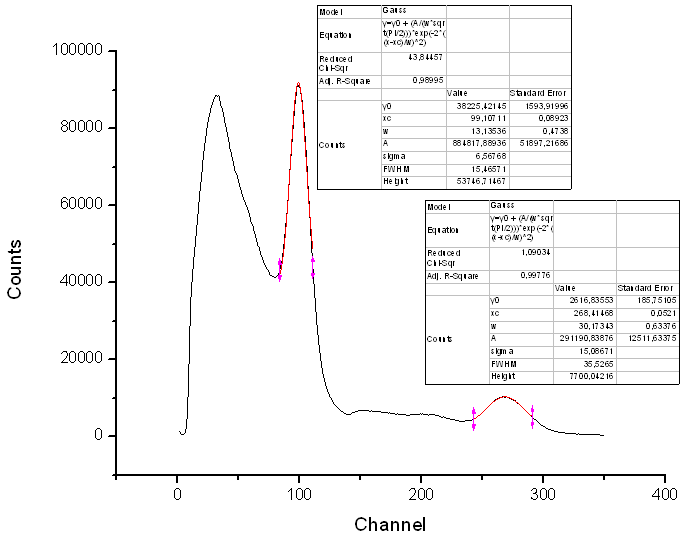
\includegraphics[width=\textwidth]{Graphen/SZ3.png}
 \caption{22Na Spektrum mit SZ3}
\end{figure}  

BLA BLA Einstellungen etc.

\subsection{Zwei-Photonen-Zerfall}

Beim Zerfall des 0S0-Singulett-Zustands des Positroniums können die Photonen, wie in der Theorie näher erläutert, nur in einem $180^\circ$-Winkel abgestrahlt werden. Dies wollen wir über eine Winkelkorrelationsmessung verifizieren. Dazu stellen wir die Szintilatoren auf ein 511keV Fenster ein und drehen SZ1 oder SZ3 gegen den festen SZ2. 
\begin{figure}
 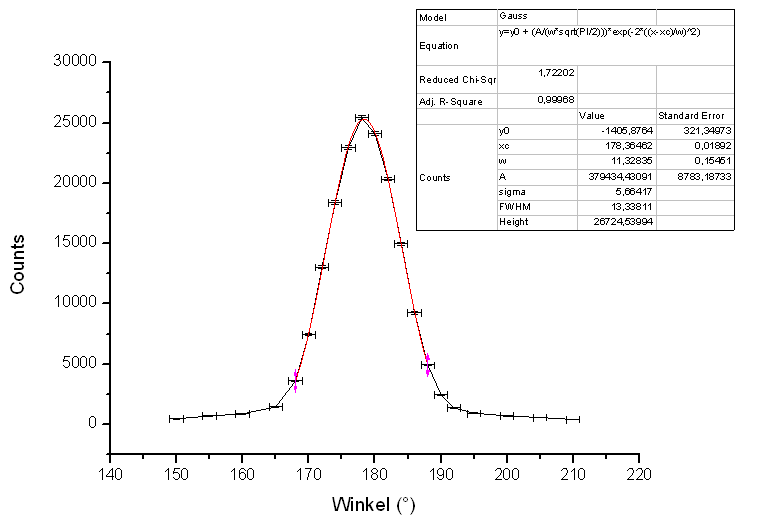
\includegraphics[width=\textwidth]{Graphen/180K.png}
 \caption{Winkelkorrelation des Zwei-Photonen-Zerfalls}
\end{figure}

\subsection{Drei-Photonen-Zerfall}

\begin{figure}
 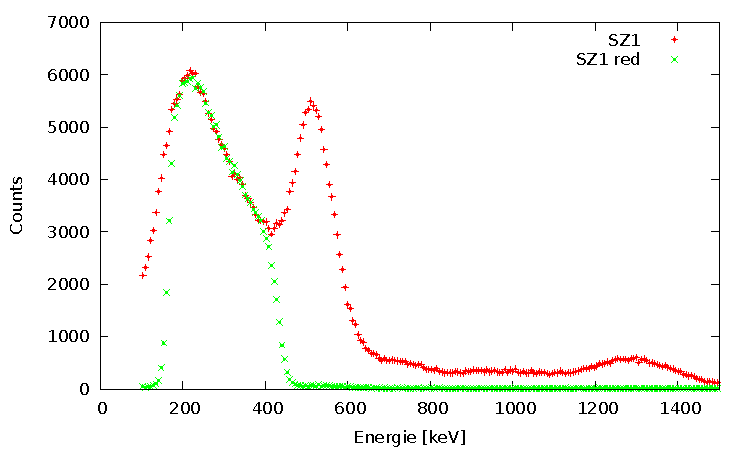
\includegraphics[width=\textwidth]{Graphen/3er/red-spektrum-sz1.pdf}
 \caption{Einstellung des Energiefensters unterhalb der 511keV-Linie für SZ1}
\end{figure}

\begin{figure}
 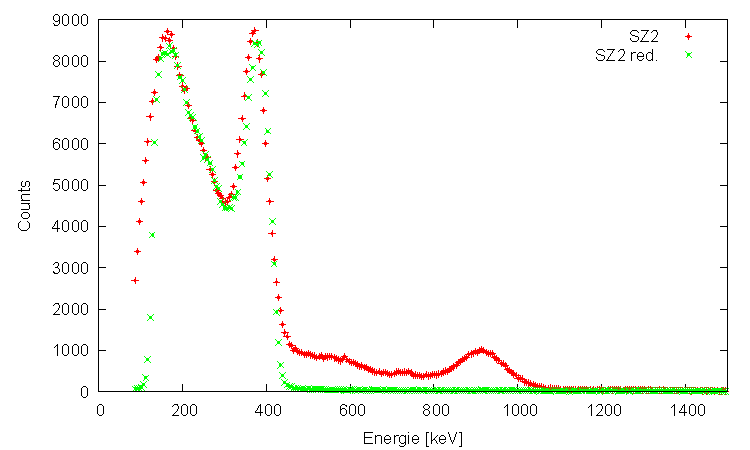
\includegraphics[width=\textwidth]{Graphen/3er/red-spektrum-sz2.pdf}
 \caption{TODO: WAS IST DAS?}
\end{figure}

\begin{figure}
 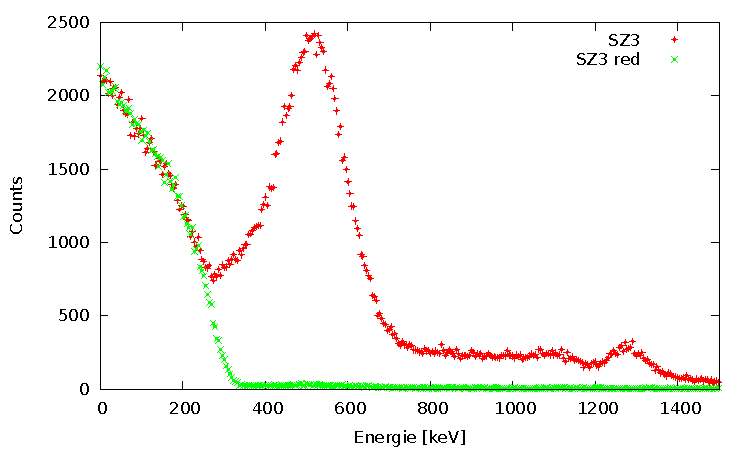
\includegraphics[width=\textwidth]{Graphen/3er/red-spektrum-sz3.pdf}
 \caption{Einstellung des Energiefensters unterhalb der 511keV-Linie für SZ3}
\end{figure}

\begin{figure}
 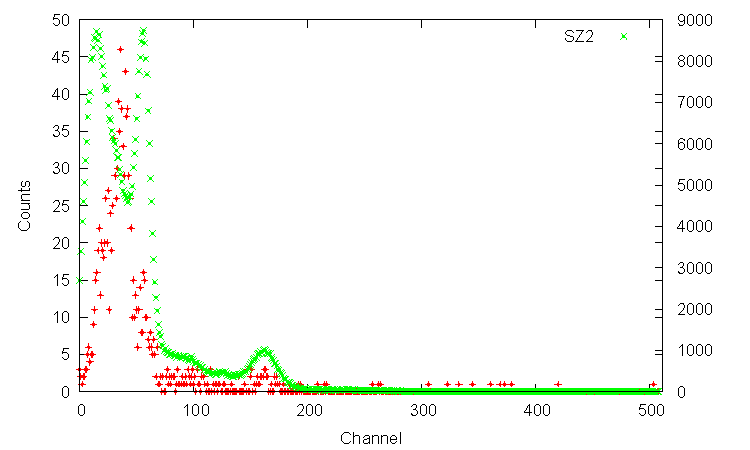
\includegraphics[width=\textwidth]{Graphen/3er/spektrum-1.pdf}
 \caption{Spektrum am SZ2 beim 3er-Koinzidenz}
\end{figure}

\begin{figure}
 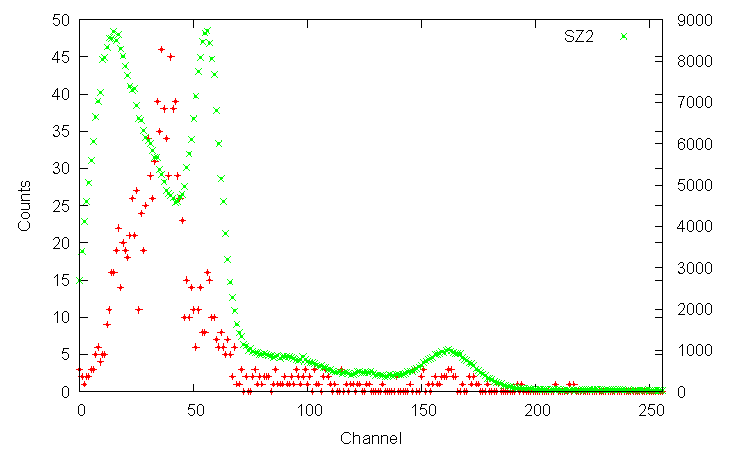
\includegraphics[width=\textwidth]{Graphen/3er/spektrum-2.pdf}
 \caption{Spektrum am SZ2 beim 3er-Koinzidenz}
\end{figure}


\subsection{Quenching}

\begin{figure}
 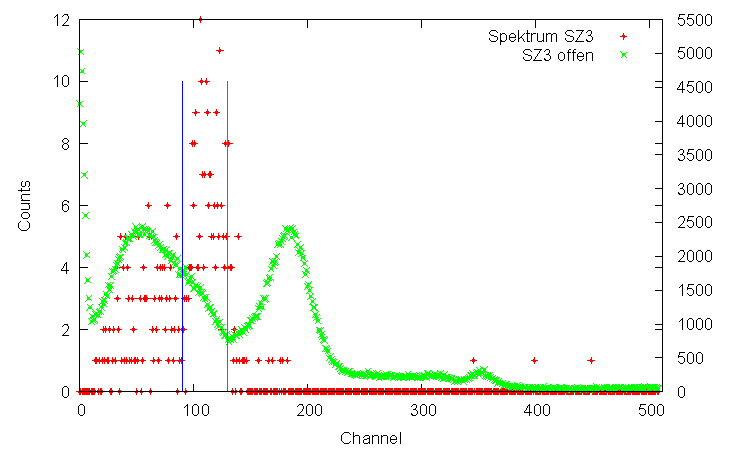
\includegraphics[width=\textwidth]{Graphen/quench/spektrum_0-3.pdf}
 \caption{Spektrum 0,3A}
\end{figure}

\begin{figure}
 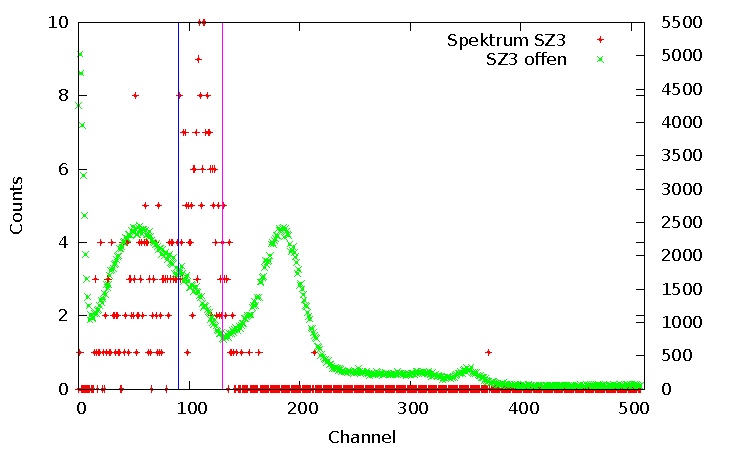
\includegraphics[width=\textwidth]{Graphen/quench/spektrum_1065.pdf}
 \caption{Spektrum 1065G}
\end{figure}


\begin{figure}
 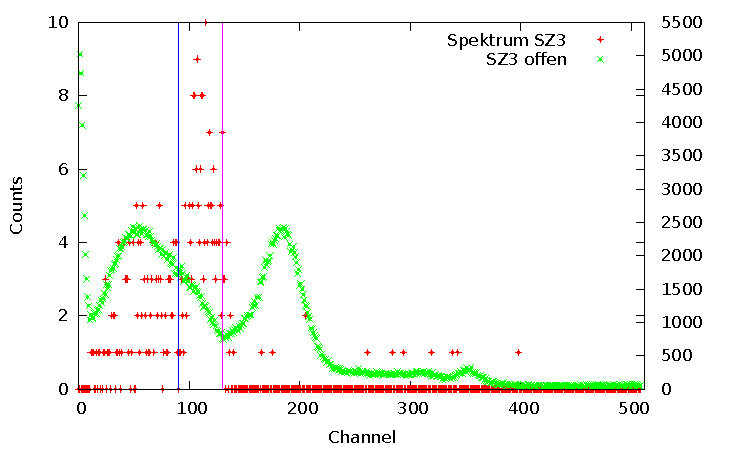
\includegraphics[width=\textwidth]{Graphen/quench/spektrum_2028.pdf}
 \caption{Spektrum 2028G}
\end{figure}


\begin{figure}
 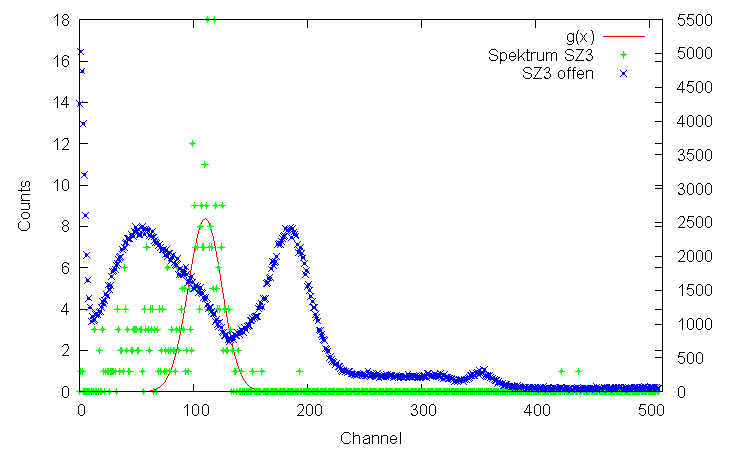
\includegraphics[width=\textwidth]{Graphen/quench/spektrum_0-3_nach_2028.pdf}
 \caption{Spektrum 0,3A nach 2028G}
\end{figure}


\begin{figure}
 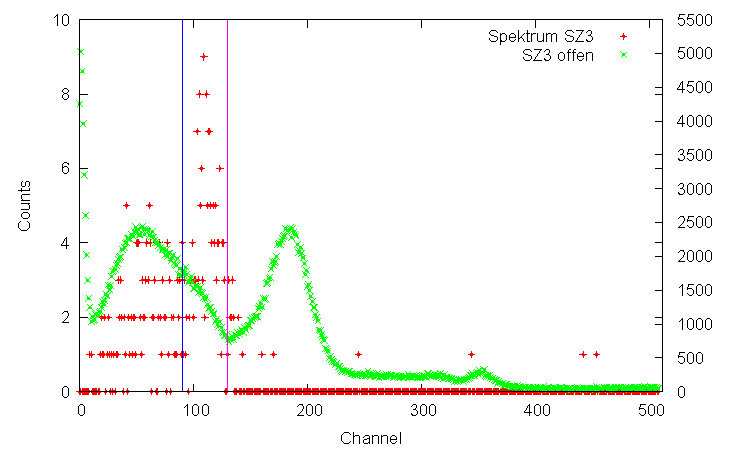
\includegraphics[width=\textwidth]{Graphen/quench/spektrum_3070.pdf}
 \caption{Spektrum 3070G}
\end{figure}

\begin{figure}
 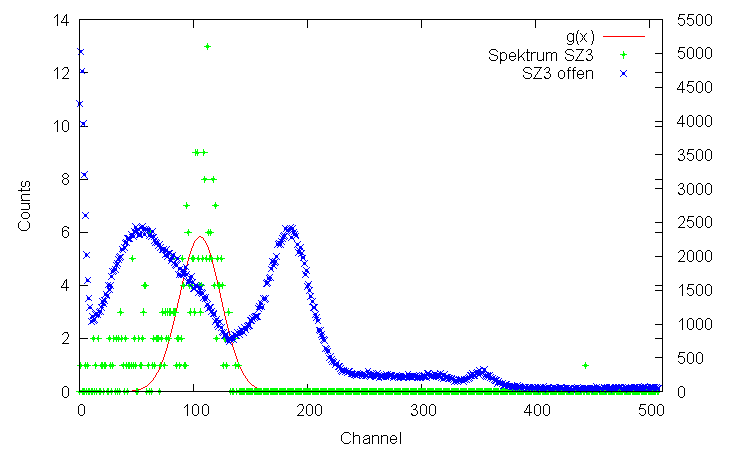
\includegraphics[width=\textwidth]{Graphen/quench/spektrum_4032.pdf}
 \caption{Spektrum 4032G}
\end{figure}

\begin{figure}
 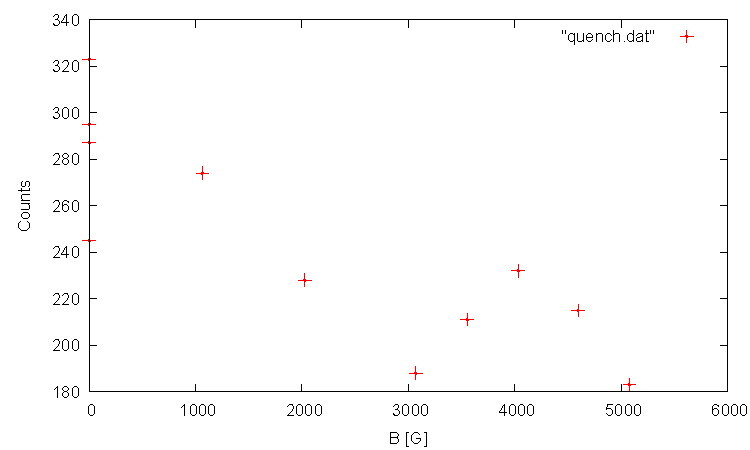
\includegraphics[width=\textwidth]{Auswertung/quench.pdf}
 \caption{Quenching des Drei-Photonen-Zerfalls in $120^\circ$-Konfiguration}
\end{figure}

\begin{figure}
 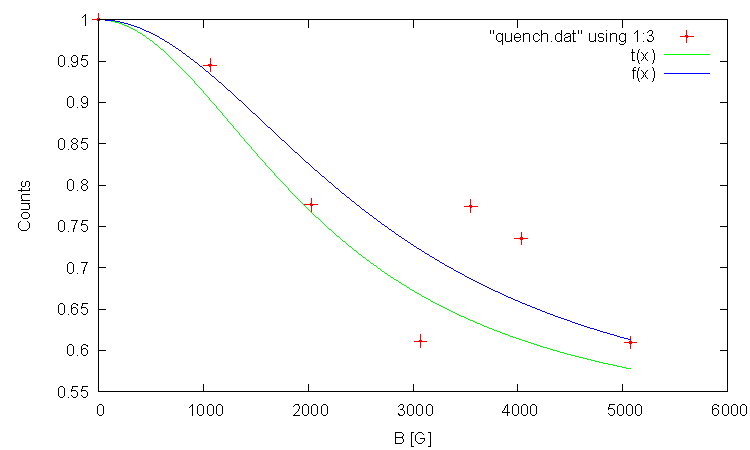
\includegraphics[width=\textwidth]{Auswertung/quench-normiert.pdf}
 \caption{Normiertes Quenching des Drei-Photonen-Zerfalls in $120^\circ$-Konfiguration}
\end{figure}
